\section{Introduction: Transparent Documents}

Making sense of and verifying data-driven claims is hard, even when the evidence base (data sets and related
analyses) is open. We see this in peer review, misinformation, retracted papers, \rpnote{supporting
citations}. The ability of LLMs to assist with these challenges has received considerable attention recently,
for example in quantity extraction~\citep{bolucu23}, scientific fact-checking~\citep{abu-ahmad25}, and
scientific figure interpretation~\citep{roberts24}.

Recent work on data provenance and data visualisation~\citep{psallidas18smoke,perera22,bond25} attempts to
address this issue through software infrastructure which transparently connections charts and figures to their
data sources. \rpnote{Contrast with LLM-based approach -- trusted infrastructure.} This enables visual outputs
to provide interactive \emph{provenance queries}, user interactions (e.g. mousing over a visual element) that
allow readers to explore how visual features relate to data. The key value proposition of these approaches is
that the interactions are provided automatically via an underlying programming language (query language or
general-purpose language) which tracks dependencies as data flows through a computation.

In this paper, we extend interactive provenance queries to the natural language that accompanies the charts
and figures. We believe this is an important step because in most articles, charts and figures usually only
play a supporting role. The main claims are usually presented in natural language, language which also makes
quantitative statements and contains substantial implicit analytic content. In principle transparent
programming languages can also be used to create natural language which is bidirectly linked to data, by
computing key fragments of natural language from data. The following example, adapted from \cite{zhang18} via
\cite{moosavi21}, shows how the language presented in this paper can be used to achieve this \rpnote{Need to
illustrate counterfactual/generalisability}:

\begin{figure}%[h]
    \centering
    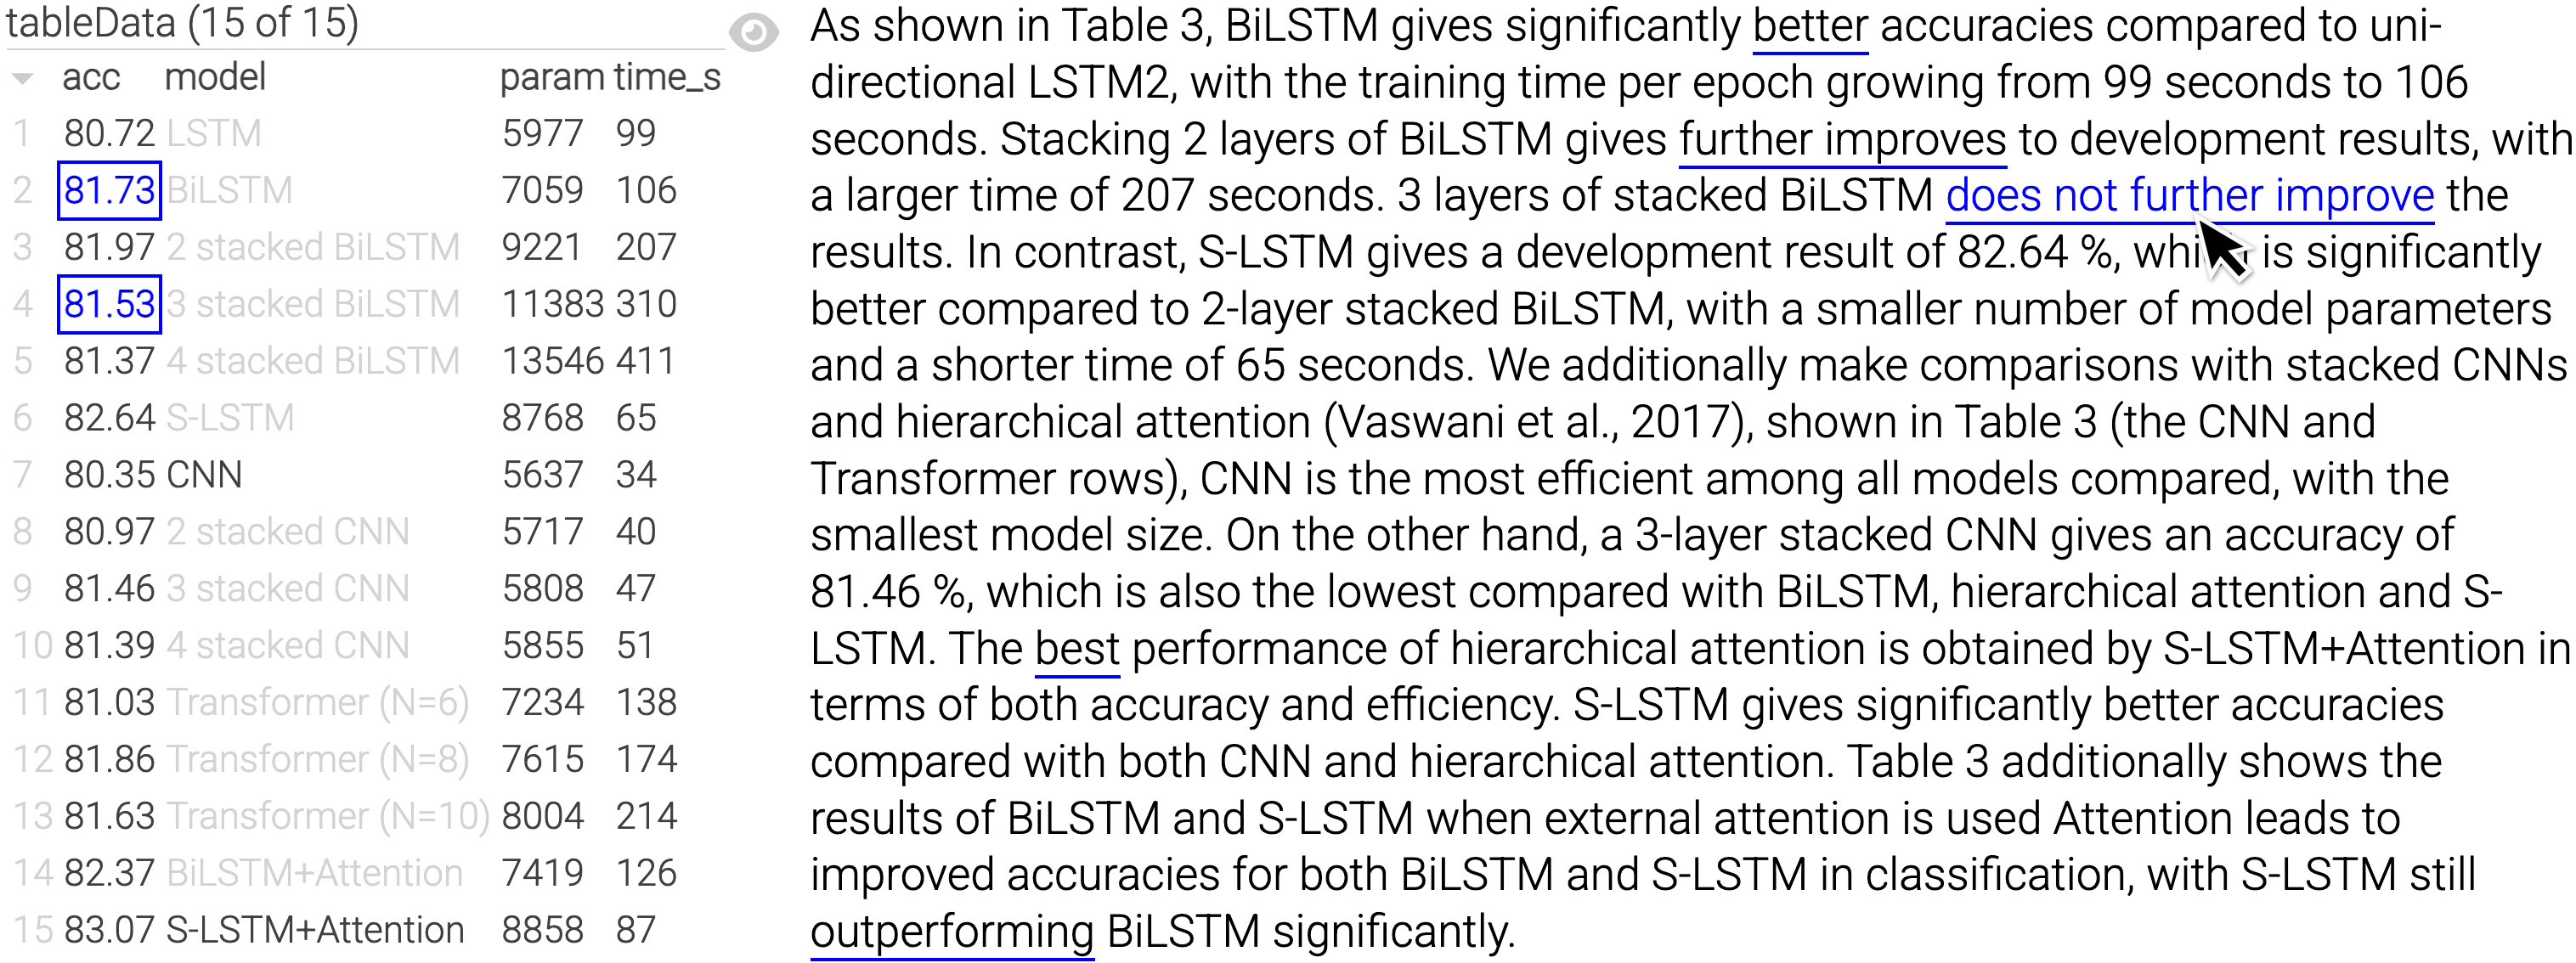
\includegraphics[width=\linewidth]{fig/scigen-1805.02474v1-10-with-pointer.png}
    \vspace{1mm}
    \hrule
    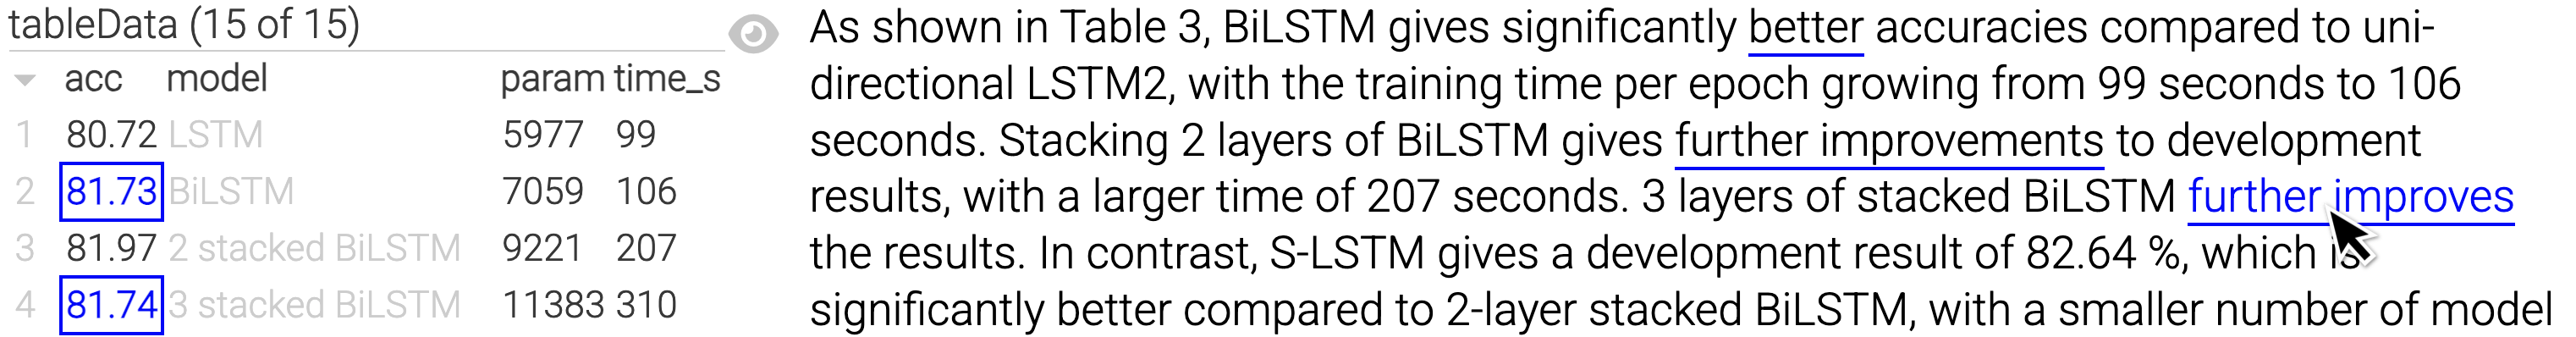
\includegraphics[width=\linewidth]{fig/scigen-1805.02474v1-10-counterfactual-with-pointer.png}
    \caption{\emph{Transparent document} example (top); counterfactual behaviour (bottom)}\label{fig:scigen-example-website}
\end{figure}

We envisage two possible use cases for transparent text:

\begin{enumerate}
\item \textbf{Authoring.} Someone authoring content for an online article, wants to create text
linked to raw data (and derivative data such as charts or tabular summaries), so that the evidence base for
the claims made in the text can be explored \emph{in situ}, by interacting with the text.

\item \textbf{Reading or reviewing.} Someone reading textual claims derived from open data (e.g. a
scientific paper or climate report), wants to retroactively link the text to queries over the available data
and gradually ``rationally reconstruct'' the relationship between the claims in the paper and the evidence
base. Perhaps just to aid their own comprehension, or to provide some kind of justified peer review.
\end{enumerate}

\begin{figure}[h]
    \small
    % listings package seems to struggle, for now just use screenshot from VSCode
    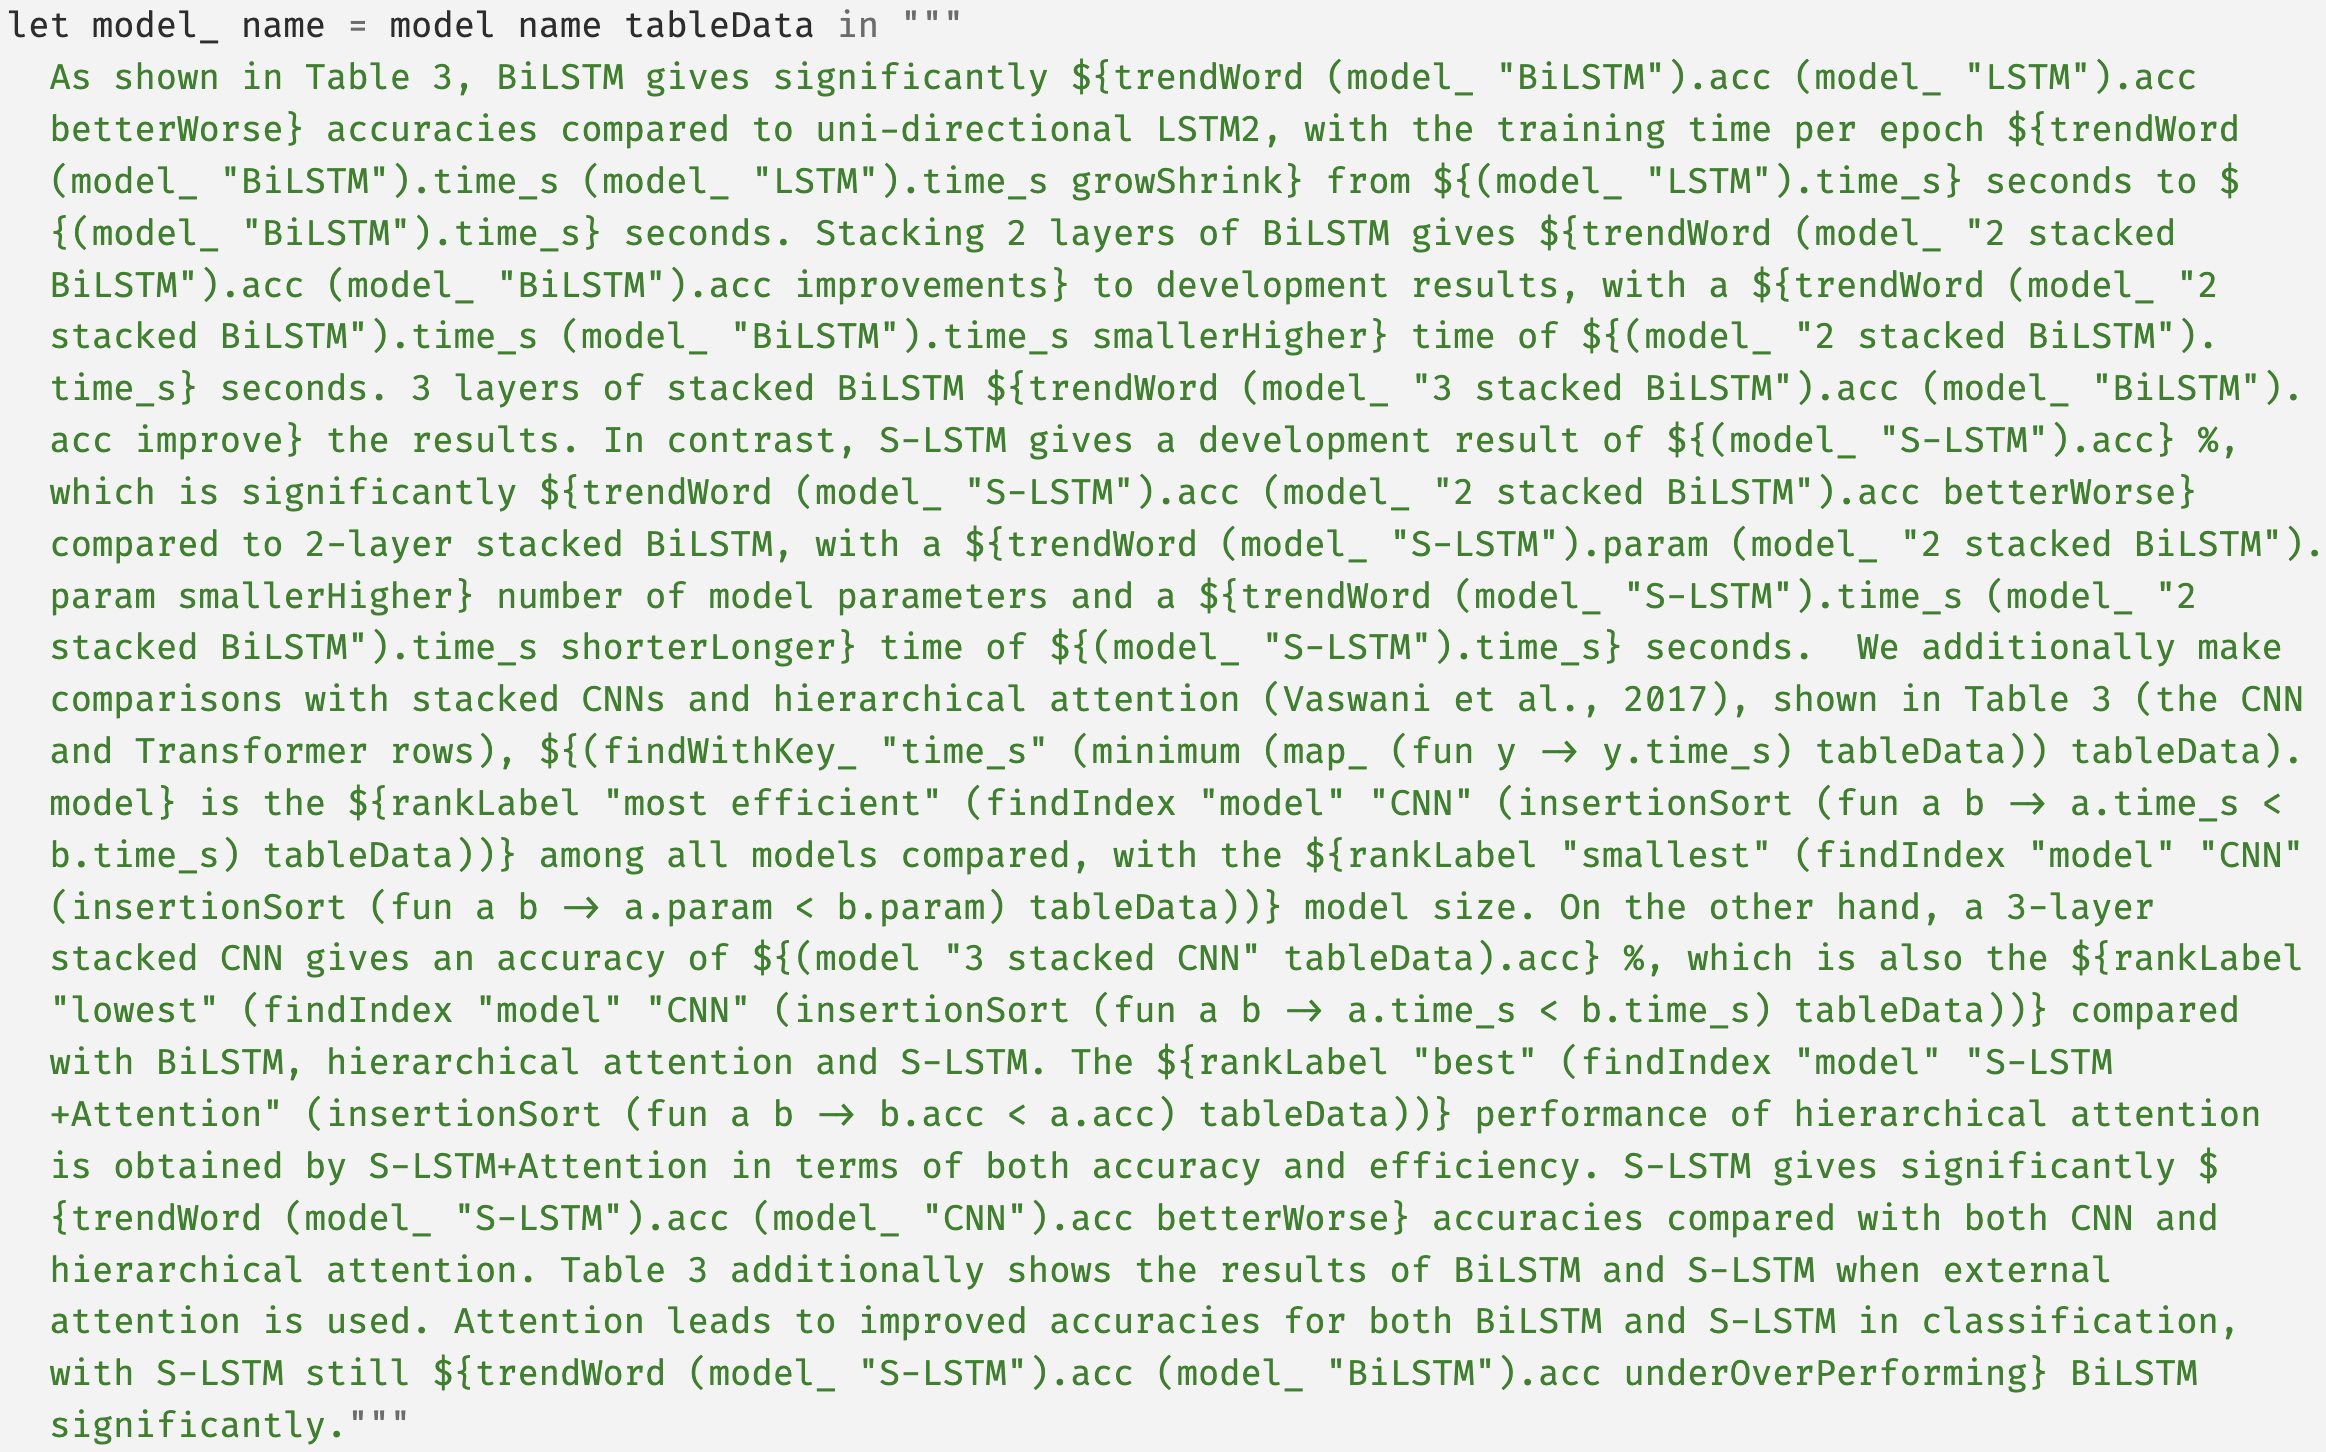
\includegraphics[scale=0.169]{fig/scigen-1805.02474v1-10-src-screenshot.png}
    \caption{Reference solution for transparent text in \figref{scigen-example-website}}
    \label{fig:fluid-example-paragraph}
\end{figure}


\subsubsection{Target idioms of natural language}

NLP aspect of the problem is potentially a big problem space in itself. We will restrict interest to certain
idiomatic uses of natural language in making/justifying scientific claims.
Examples \ref{tab:fluid_examples}

\begin{table}[!ht]
    \centering
    \footnotesize
    \renewcommand{\arraystretch}{1.2}
    \begin{tabular}{>{\raggedright\arraybackslash}p{2cm} >{\raggedright\arraybackslash}p{5cm} >{\raggedright\arraybackslash}p{6cm}}
        \hline
        \textbf{Type}                & \textbf{Example} & \textbf{Generated Expression} \\
        \rowcolor{gray!20}
        \multicolumn{3}{>{\raggedright\arraybackslash}l}{\textbf{Quantitative expressions}} \\

        Numerical value
        & the training time per epoch growing from \hl{67} seconds to 106 seconds.
        &
        \begin{lstlisting}[language=Fluid,numbers=none]
(findWithKey' "model" "LSTM" tableData).time_s
        \end{lstlisting}
        \\
        Percentage &
        The Energy Sector accounts for total methane emissions of \hl{52.80\%} in 2030.
        &
        \begin{lstlisting}[language=Fluid,numbers=none]
(record.emissions /
 sum (map (fun x -> x.emissions)
          (getByYear year tableData))) * 100

        \end{lstlisting}  \\
        Rounding* & about 2 degrees warmer                & ~                             \\
        Cardinal* & three                & ~                             \\
        Multiplicative* & three times                & ~                             \\
        \rowcolor{gray!20}
        \multicolumn{3}{>{\raggedright\arraybackslash}l}{\textbf{Aggregation}} \\
        Average
        & The average methane emissions for the year 2030 is \hl{13.51} &
        \begin{lstlisting}[language=Fluid,numbers=none]
(sumEmissions year tableData / length records)
        \end{lstlisting} \\
        Min/Max                          & The Energy Sector recorded its highest methane emissions in \hl{2030}             &
        \begin{lstlisting}[language=Fluid,numbers=none]
let maxEntry =
    maximumBy (fun x -> x.emissions)
              (filter
                (fun x -> x.type == "Energy Sector")
                tableData)
in maxEntry.year
        \end{lstlisting} \\                             \\
        Rank &
        3-layer stacked CNN gives an accuracy of 81.46\%, which is the \hl{lowest} compared with BiLSTM, and S-LSTM  &
        \begin{lstlisting}[language=Fluid,numbers=none]
let pos =
  findIndex "model" "CNN"
    (insertionSort cmpTime tableData)
in rankLabel "lowest" pos \end{lstlisting} \\
        Total &
        The total methane emissions for the year 2030 is \hl{37.74} for Agriculture &
        \begin{lstlisting}[language=Fluid,numbers=none]
sumEmissions year tableData
        \end{lstlisting} \\
        Count*                       & ~                & ~                             \\
        \rowcolor{gray!20}
        \multicolumn{3}{>{\raggedright\arraybackslash}l}{\textbf{Trends}} \\

        Comparison
        & The training time per epoch \hl{growing} from 67 seconds to 106 seconds. &
        \begin{lstlisting}[language=Fluid,numbers=none]
trendWord
 (findWithKey' "model" "BiLSTM" tableData).time_s
 (findWithKey' "model" "LSTM" tableData).time_s
 growShrink
        \end{lstlisting} \\
        Graded adjective*            & \hl{extremely likely} to be exceeded in the 20th century               & ~                             \\
        Reference to visual element*                            & ~                & ~                             \\
        \hline
    \end{tabular}
    \caption{Quantitative/semi-quantitative natural language forms considered in this paper}
    \label{tab:fluid_examples}
\end{table}


\subsection{Contributions}

\begin{itemize}
    \item Design and proof-of-concept implementation of AI-assisted workflow for authoring transparent text
    (\secref{authoring-workflow})
    \item Empirical evaluation of how effective current LLMs are at providing the ``AI-assisted'' part
\end{itemize}
